\documentclass[xcolor=dvipsnames]{beamer}
\makeatletter\def\Hy@xspace@end{}\makeatother 
\usepackage{graphicx, color, amssymb, amsmath, bm, rotating, graphics,
epsfig, multicol, amsthm, animate}
\usepackage[english]{babel}
\usepackage[T1]{fontenc}
\usepackage[ansinew]{inputenc}
\usepackage[authoryear]{natbib}
%\newcommand{\newblock}{}  %needed to make beamer and natbib play nice
\usepackage{tikz, caption}
% A counter, since TikZ is not clever enough (yet) to handle
% arbitrary angle systems.
\newcount\mycount

\usetheme{Boadilla}
%\usecolortheme{lily}
\definecolor{MUgold}{RGB}{241,184,45}
\usecolortheme[named=MUgold]{structure}
\setbeamercolor{structure}{bg=Black}
\setbeamercolor{structure}{fg=MUgold}
\setbeamercolor{title}{bg=Black}
\setbeamercolor{frametitle}{bg=Black, fg=MUgold}
\setbeamercolor{title in head/foot}{fg=Black, bg=MUgold}
\setbeamercolor{author in head/foot}{fg=MUgold, bg=Black}
\setbeamercolor{institute in head/foot}{fg=MUgold, bg=Black}
\setbeamercolor{date in head/foot}{fg=MUgold, bg=Black}
\setbeamercolor{item projected}{bg=MUgold, fg=Black}
\usesubitemizeitemtemplate{\tiny\raise1.5pt\hbox{\color{Black}$\blacktriangleright$}}
\setbeamercovered{transparent=0}
\beamertemplatenavigationsymbolsempty

\title[PSO for MCMC]{Particle Swarm Optimization Assisted Markov Chain Monte Carlo}

%\subtitle{}
\author[Matt Simpson]{Matthew Simpson}
\institute[Mizzou Statistics]{Department of Statistics, University of Missouri}
\date{August 3, 2016}

\begin{document}

\begin{frame}
\titlepage
\centering
{\scriptsize
Joint work with Christopher Wikle and Scott H. Holan\\~\\
Research supported by the NSF-Census Research Network}
\end{frame}

\begin{frame}
\frametitle{Particle Swarm Optimization}
Finding MLE for an $iid$ beta model. Red point = true MLE.
\centering
\animategraphics[autoplay,loop,width=0.6\linewidth]{2}{animplot}{1}{25}
\end{frame}


% \begin{frame}
% \frametitle{Goals \& Outline}
% Goal 1: construct efficient MCMC algorithms for posterior sampling.
% \begin{enumerate}
% \item Use particle swarm optimization (PSO) to estimate posterior modes.
% \item Use a mode based approximation (Laplace) as a proposal for independent Metropolis and independent Metropolis within Gibbs.\\~\\
% \end{enumerate}
% Goal 2: develop improved PSO algorithms by borrowing tuning methods from adaptive MCMC.\\~\\

% Outline:
% \begin{enumerate}
% \item Generic PSO algorithms.
% \item Adaptively tuned PSO algorithms.
% \item Laplace approximations and Metropolis algorithms based on them.
% \item Example: spatially modeling ACS county population estimates.
% \end{enumerate}
% \end{frame}

\begin{frame}
\frametitle{Particle Swarm Optimization}
Goal: maximize $Q(\bm{\theta}): \Theta \to \Re$; $\Theta \subseteq \Re^D$.\\~\\
Populate $\Theta$ with $n_{part}$ particles. Define particle $i$ in period $t$ by:
\begin{itemize}
\item a location $\bm{\theta}_i(t)\in \Theta$;
\item a velocity $\bm{v}_i(t) \in \Theta$;
\item a personal best location $\bm{p}_i(t) \in \Theta$: $Q(\bm{p}_i(t))\geq Q(\bm{\theta}_i(s))$ for $s\leq t$;
\item a group best location \hspace{0.28cm} $\bm{g}_i(t) \in \Theta$: $Q(\bm{g}_i(t))\geq Q(\bm{\theta}_i(s))$ for $s\leq t$.\\~\\
\end{itemize}
 Update particle $i$ from $t$ to $t+1$ via: for $j=1,2,\dots,D$
{\color{black}
\begin{align*}
v_{ij}(t+1) &= \omega v_{ij}(t) +  U(0,\phi_1)\times\{p_{ij}(t) - \theta_{ij}(t)\} \\
     &\;\phantom{= \omega v_{ij}(t)}+  U(0,\phi_2)\times\{g_{ij}(t) - \theta_{ij}(t)\}\\
& = \mbox{inertia} + \mbox{cognitive} + \mbox{social},\\
\theta_{ij}(t+1) &= \theta_{ij}(t) + v_{ij}(t+1),
\end{align*}}
Default choices: $\omega=0.7298$, $\phi_1=\phi_2=1.496$ \\
\ \ \ \ \ \citep{clerc2002particle,blum2008swarm}
\end{frame}


\begin{frame}
\frametitle{PSO --- Neighborhood Topologies}
Sometimes it is useful to restrict the flow of information across the swarm --- e.g. complicated objective functions with many local optima.\\~\\

 Ring-$k$ neighborhood topology: arrange particles in a ring; each particle has $k$ neighbors to the left and $k$ to the right.

        \begin{figure}
          \centering
          {
            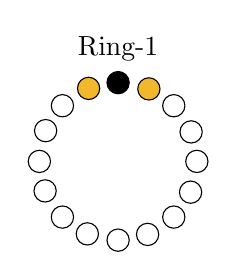
\begin{tikzpicture}[transform shape]
              % the multiplication with floats is not possible. Thus I split the loop in two.
              \foreach \number in {1,...,2}{
                % Computer angle:
                \mycount=\number
                \advance\mycount by 0
                \multiply\mycount by 45
                \advance\mycount by 22.5
                \node[circle,inner sep=0.1cm,fill=MUgold] (N-\number) at (\the\mycount:1cm) {};
              }
              \foreach \number in {1,...,1}{
                % Computer angle:
                \mycount=\number
                \advance\mycount by 1
                \multiply\mycount by 45
                \advance\mycount by 0
                \node[draw=black,circle,inner sep=0.1cm,fill=black,label=Ring-1] (N-\number) at (\the\mycount:1cm) {};
              \foreach \number in {1,...,7}{
                % Computer angle:
                \mycount=\number
                \advance\mycount by 2
                \multiply\mycount by 45
                \advance\mycount by 0
                \node[draw,circle,inner sep=0.1cm] (N-\number) at (\the\mycount:1cm) {};
              }
              \foreach \number in {8,...,15}{
                % Computer angle:
                \mycount=\number
                \advance\mycount by 1
                \multiply\mycount by 45
                \advance\mycount by 22.5
                \node[draw,circle,inner sep=0.1cm] (N-\number) at (\the\mycount:1cm) {};
              }
              }
            \end{tikzpicture}
          }
          {
            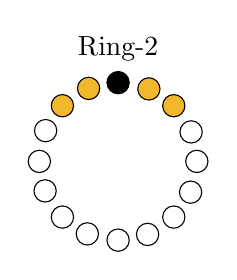
\begin{tikzpicture}[transform shape]
              % the multiplication with floats is not possible. Thus I split the loop in two.
              \foreach \number in {1,...,2}{
                % Computer angle:
                \mycount=\number
                \advance\mycount by 0
                \multiply\mycount by 45
                \advance\mycount by 22.5
                \node[circle,inner sep=0.1cm,fill=MUgold] (N-\number) at (\the\mycount:1cm) {};
              }
              \foreach \number in {1,...,3}{
                % Computer angle:
                \mycount=\number
                \advance\mycount by 0
                \multiply\mycount by 45
                \advance\mycount by 0
                \node[circle,inner sep=0.1cm,fill=MUgold] (N-\number) at (\the\mycount:1cm) {};
              }
              \foreach \number in {1,...,1}{
                % Computer angle:
                \mycount=\number
                \advance\mycount by 1
                \multiply\mycount by 45
                \advance\mycount by 0
                \node[draw=black,circle,inner sep=0.1cm,fill=black,label=Ring-2] (N-\number) at (\the\mycount:1cm) {};
              \foreach \number in {1,...,7}{
                % Computer angle:
                \mycount=\number
                \advance\mycount by 2
                \multiply\mycount by 45
                \advance\mycount by 0
                \node[draw,circle,inner sep=0.1cm] (N-\number) at (\the\mycount:1cm) {};
              }
              \foreach \number in {8,...,15}{
                % Computer angle:
                \mycount=\number
                \advance\mycount by 1
                \multiply\mycount by 45
                \advance\mycount by 22.5
                \node[draw,circle,inner sep=0.1cm] (N-\number) at (\the\mycount:1cm) {};
              }
              }
            \end{tikzpicture}
          }
          {
            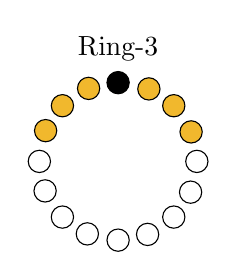
\begin{tikzpicture}[transform shape]
              % the multiplication with floats is not possible. Thus I split the loop in two.
              \foreach \number in {1,...,4}{
                % Computer angle:
                \mycount=\number
                \advance\mycount by -1
                \multiply\mycount by 45
                \advance\mycount by 22.5
                \node[circle,inner sep=0.1cm,fill=MUgold] (N-\number) at (\the\mycount:1cm) {};
              }
              \foreach \number in {1,...,3}{
                % Computer angle:
                \mycount=\number
                \advance\mycount by 0
                \multiply\mycount by 45
                \advance\mycount by 0
                \node[circle,inner sep=0.1cm,fill=MUgold] (N-\number) at (\the\mycount:1cm) {};
              }
              \foreach \number in {1,...,1}{
                % Computer angle:
                \mycount=\number
                \advance\mycount by 1
                \multiply\mycount by 45
                \advance\mycount by 0
                \node[draw=black,circle,inner sep=0.1cm,fill=black,label=Ring-3] (N-\number) at (\the\mycount:1cm) {};
              \foreach \number in {1,...,7}{
                % Computer angle:
                \mycount=\number
                \advance\mycount by 2
                \multiply\mycount by 45
                \advance\mycount by 0
                \node[draw,circle,inner sep=0.1cm] (N-\number) at (\the\mycount:1cm) {};
              }
              \foreach \number in {8,...,15}{
                % Computer angle:
                \mycount=\number
                \advance\mycount by 1
                \multiply\mycount by 45
                \advance\mycount by 22.5
                \node[draw,circle,inner sep=0.1cm] (N-\number) at (\the\mycount:1cm) {};
              }
              }
            \end{tikzpicture}
          }
          {
            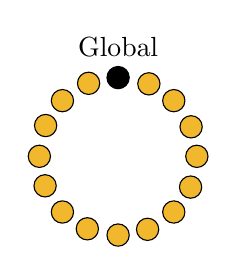
\begin{tikzpicture}[transform shape]
              % the multiplication with floats is not possible. Thus I split the loop in two.
              \foreach \number in {2,...,8}{
                % Computer angle:
                \mycount=\number
                \advance\mycount by 1
                \multiply\mycount by 45
                \advance\mycount by 0
                \node[draw,circle,inner sep=0.1cm,fill=MUgold] (N-\number) at (\the\mycount:1cm) {};
              }
              \foreach \number in {9,...,16}{
                % Computer angle:
                \mycount=\number
                \advance\mycount by 1
                \multiply\mycount by 45
                \advance\mycount by 22.5
                \node[draw,circle,inner sep=0.1cm,fill=MUgold] (N-\number) at (\the\mycount:1cm) {};
              }
              \foreach \number in {1,...,1}{
                % Computer angle:
                \mycount=\number
                \advance\mycount by 1
                \multiply\mycount by 45
                \advance\mycount by 0
                \node[draw=black,circle,inner sep=0.1cm,fill=black,label=Global] (N-\number) at (\the\mycount:1cm) {};
              }
            \end{tikzpicture}
          }
          \caption*{Filled in gold particles are neighbors of the filled in black particle.}
        \end{figure}
\end{frame}

\begin{frame}
\frametitle{Adaptively Tuning PSO}
In PSO larger $\omega$ $\implies$ more exploration, smaller $\omega$ $\implies$ more exploitation.\\~\\

Idea: slowly decrease $\omega(t)$ over time \citep{eberhart2000comparing}.\\~\\

 AT-PSO: tune $\omega(t)$ like in adaptive MCMC \citep{andrieu2008tutorial}.
\begin{itemize}
\item Define the swarm's improvement rate:
\begin{align*}
R(t) = \frac{\left|\left\{i:Q[\bm{p}_i(t)] > Q[\bm{p}_i(t-1)]\right\}\right|}{n}.
\end{align*}
and let $R^*$ be the target rate.
\item Then update: $\log\omega(t+1) = \log\omega(t) + c\times\mbox{sgn}\{R(t) - R^*\}$.
\end{itemize}
Good choices: $c=0.1$ and $R^*=0.5$.\\~\\

 Tuning $\omega(t)$ allows the swarm to adjust the exploration / exploitation tradeoff based on local conditions.
\begin{itemize}
\item This has a tendency to speed up convergence.
\item ...but convergence may be premature in multi-modal problems.
\end{itemize}
\end{frame}

% \begin{frame}
% \frametitle{General PSO Recommendations}
% AT-PSO with $c=0.1$ and $R^*=0.5$ tends to be the fastest PSO variant.
% \vspace{0.3cm}
% \begin{itemize}
% \item Often other variants are competitive and occasionally even better.
% \vspace{0.3cm}
% \item Use a small number of iterations of a gradient based algorithm to initialize the PSO algorithm (e.g. BFGS).\\~\\
% \end{itemize}

% \vspace{0.5cm}

% PSO is generally more robust than gradient based alternatives, but when a gradient based method works it will generally be faster.
% \vspace{0.3cm}
% \begin{itemize}
% \item PSO is often used for optimizing difficult objective functions (e.g. neural nets, knot selection, design problems), and for multi-objective optimization.
% \end{itemize}

% \end{frame}

\begin{frame}
\frametitle{Laplace Approximation to the Posterior}
Posterior distribution: $p(\bm{\theta}|\bm{y}_{1:n})$. Let $\bm{\theta}^*_n$ be the posterior mode\\
 and let $\bm{H}_n(\bm{\theta}^*_n)$ denote the Hessian of $\log p(\bm{\theta}|\bm{y}_{1:n})$ evaluated at $\bm{\theta}^*_n$.\\~\\

Laplace approximation \citep[Sections~7.4.2~and~7.4.3]{schervish1997theory}: 
\begin{align*}
\bm{\theta}|\bm{y}_{1:n} \stackrel{a}{\sim} N(\bm{\theta}_n^*, -\bm{H}_n^{-1}(\bm{\theta}^*_n)) && \mbox{for large }n.
\end{align*}

%  This approximation is more likely to be good when:
% \begin{itemize}
% \item each parameter has a lot of relevant ``observations'' --- e.g. many random effects for a variance.
% \item the data and process models are (approximately) Gaussian.\\~\\
% \end{itemize}
\vspace{0.5cm}
 Standard usage: proposal for independent Metropolis-Hastings (IMH).\\
\begin{itemize}
\item Use $t_{df}$ kernel to ensure the proposal's tails dominate the posterior's.
\item Use PSO (or some other optimization algorithm) to find $\bm{\theta}^*_n$.
\end{itemize}


\end{frame}

\begin{frame}
\frametitle{Laplace Approximation for IMH within Gibbs}
Let $\bm{\theta}=(\bm{\theta}_1,\bm{\theta}_2)$ and $\bm{\Sigma}^* = [-\bm{H}^*(\bm{\theta}^*_n)]^{-1} = \begin{bmatrix} \bm{\Sigma}^*_{11} & \bm{\Sigma}^*_{12} \\ \bm{\Sigma}^*_{21} & \bm{\Sigma}^*_{22} \end{bmatrix}$.\\~\\

Suppose $p(\bm{\theta}_2|\bm{\theta}_1, \bm{y}_{1:n})$ is easy to draw from and $p(\bm{\theta}_1|\bm{\theta}_2, \bm{y}_{1:n})$ is approximately Gaussian.  Then IMH within Gibbs (IMHwG) may work well:
\begin{enumerate}
\item Draw $\bm{\theta}_2^{(t+1)} \sim p(\bm{\theta}_2|\bm{\theta}_1^{(t)},\bm{y}_{1:n})$.
\item Metropolis step with proposal $\bm{\theta}_1^{prop}\sim t_{df}(\widetilde{\bm{\theta}}_1, \widetilde{\bm{\Sigma}}_{11})$, where 
\begin{align*}
\widetilde{\bm{\theta}}_1 &= \bm{\theta}_1^* + \bm{\Sigma}_{12}^*(\bm{\Sigma}_{22}^*)^{-1}(\bm{\theta}_2^{(t+1)} - \bm{\theta}_2^*),\\ 
\widetilde{\bm{\Sigma}}_{11} &= \bm{\Sigma}_{11}^* - \bm{\Sigma}_{12}^*(\bm{\Sigma}_{22}^*)^{-1}\bm{\Sigma}_{21}^*.
\end{align*}
\end{enumerate}
Uses a global Laplace approx to construct an approx for $p(\bm{\theta}_1|\bm{\theta}_2,\bm{y}_{1:n})$.
\begin{itemize}
\item Worse than directly approximating $p(\bm{\theta}_1|\bm{\theta}_2,\bm{y}_{1:n})$.
\item But for MCMC, it is much cheaper to do the optimization once rather than every iteration.
\end{itemize}
\end{frame}

\begin{frame}
\frametitle{Spatial Models of County Population Estimates}
The American Community Survey (ACS) provides 5-year period estimates of county populations as recently as 2014.\\~\\
In 2014 there were $n=3,142$ counties in the United States, including the District of Columbia, Alaska, and Hawaii.\\~\\

 Let $Z_i$ denote the ACS estimate of the population of county $i$ and $Y_i$ denote the true population. Data models:
\begin{enumerate}
\item  Poisson: $Z_i|\bm{Y}_{1:n} \sim Pois\left(Y_i\right)$.
%\item  lognormal: $\log Z_i|\bm{Y}_{1:n} \sim N\left(\log Y_i,\phi^2\right)$.\\~\\
\end{enumerate}
Process model:
\begin{align*}
\log\bm{Y}_{1:n} &= \bm{X}\bm{\beta} + \bm{S}\bm{\delta} = \mbox{fixed effects} + \mbox{random effects},
\end{align*}
where $\bm{X}$ is a $n\times p$ matrix of covariates and $\bm{S}$ is a $n\times r$ matrix of spatial basis functions.
\end{frame}

\begin{frame}
\frametitle{Spatial Models of County Population Estimates}
\framesubtitle{Process model details}
\vspace{-0.6cm}
\begin{align*}
\log\bm{Y}_{1:n} &= \bm{X}\bm{\beta} + {\color{red}\bm{S}\bm{\delta}}
\end{align*}
Define $\bm{G}=(\bm{I}_n - \bm{X}(\bm{X}'\bm{X})^{-1}\bm{X}')\bm{A}(\bm{I}_n - \bm{X}(\bm{X}'\bm{X})^{-1}\bm{X}')$.\\
\begin{itemize}
\item[] $\bm{A}$ is the binary adjacency matrix: $a_{ij} = 1$ if counties $i$ and $j$ are neighbors, $a_{ij}=0$ otherwise, and $a_{ii}=0$ along the diagonal.\vspace{0.3cm}
\end{itemize}
$\bm{S}$ is the $r$ eigenvectors corresponding to the largest $r$ eigenvalues of $\bm{G}$.
\begin{itemize}
\item Forces the spatial model onto the residual variation of $\log \bm{Y}_{1:n}$.
\item Known as the truncated Moran's I basis set.
\item\citet{hughes2013dimension,porter2015bayesian,bradley2015multivariate}.\vspace{0.3cm}
\end{itemize}

Choose $r\ll n$ so the model is reduced rank (use sensitivity analysis). \vspace{0.3cm}

 Random effects models:
\begin{enumerate}
\item iid random effects: $\delta_i\stackrel{iid}{\sim}N(0,\sigma^2)$,
\item fully correlated random effects: $\bm{\delta}\sim N(\bm{0},\bm{\Sigma})$.
\end{enumerate}
\end{frame}

%\setbeamerfont{frametitle}{size=\tiny}
\begin{frame}
\frametitle{IMH AND IMHwG acceptance rates}
% \vspace{-0.2cm}
% {\small \hfill IMH and IMHwG acceptances rates for Poisson models \hfill}

% \vspace{0.2cm}

\centering
\resizebox{.4\textwidth}{!}{
\begin{tabular}{rrrrrr}
\multicolumn{6}{c}{IMH;  iid random effects, r = 10}\\
  \hline
$n_{iter}$ & PSO & DI-PSO & BBPSO & AT-BB & AT-PSO \\ 
  \hline
100   & 0.28 & 0.28 & 0.37 & 0.33 & 0.65 \\ 
500   & 0.88 & 0.89 & 0.27 & 0.23 & 0.89 \\ 
1000  & 0.89 & 0.89 & 0.32 & 0.28 & 0.89 \\ 
1500  & 0.89 & 0.89 & 0.29 & 0.29 & 0.88 \\ 
2000  & 0.89 & 0.89 & 0.27 & 0.31 & 0.89 \\ 
   \hline
\end{tabular}
}
\resizebox{.4\textwidth}{!}{
\begin{tabular}{rrrrrr}
\multicolumn{6}{c}{IMHwG;  iid random effects, r = 10}\\
  \hline
$n_{iter}$ & PSO & DI-PSO & BBPSO & AT-BB & AT-PSO \\ 
  \hline
100 &  0.45 & 0.03 & 0.04 & 0.04 & 0.21 \\ 
  500  & 0.97 & 0.97 & 0.05 & 0.02 & 0.97 \\ 
  1000  & 0.97 & 0.96 & 0.09 & 0.05 & 0.97 \\ 
  1500  & 0.96 & 0.97 & 0.10 & 0.10 & 0.97 \\ 
  2000  & 0.96 & 0.96 & 0.01 & 0.01 & 0.97 \\ 
   \hline
\end{tabular}
}\\~\\\vspace{0.3cm}

\resizebox{.4\textwidth}{!}{
\begin{tabular}{rrrrrr}
\multicolumn{6}{c}{IMH; fully correlated random effects, r = 5}\\
  \hline
$n_{iter}$ &  PSO & DI-PSO & BBPSO & AT-BB & AT-PSO \\ 
  \hline
100 & 0.04 & 0.03 & 0.07 & 0.04 & 0.02 \\ 
  500 & 0.04 & 0.20 & 0.01 & 0.08 & 0.18 \\ 
  1000 & 0.35 & 0.29 & 0.04 & 0.03 & 0.45 \\ 
  1500 & 0.33 & 0.40 & 0.01 & 0.03 & 0.34 \\ 
  2000 & 0.24 & 0.37 & 0.06 & 0.05 & 0.40 \\ 
   \hline
\end{tabular}
}
\resizebox{.4\textwidth}{!}{
\begin{tabular}{rrrrrr}
\multicolumn{6}{c}{IMHwG; fully correlated random effects, r = 5}\\
  \hline
$n_{iter}$ & PSO & DI-PSO & BBPSO & AT-BB & AT-PSO \\ 
  \hline
100 & 0.24 & 0.35 & 0.25 & 0.23 & 0.48 \\ 
  500 & 0.31 & 0.71 & 0.31 & 0.31 & 0.86 \\ 
  1000 & 0.85 & 0.97 & 0.36 & 0.54 & 0.98 \\ 
  1500 & 0.97 & 0.98 & 0.29 & 0.63 & 0.98 \\ 
  2000 & 0.97 & 0.97 & 0.47 & 0.33 & 0.97 \\ 
   \hline
\end{tabular}
}
\end{frame}
%\setbeamerfont{frametitle}{size=\Large}

% \begin{frame}
% \frametitle{Spatials Models of County Population Estimates}
% \framesubtitle{Lessons from acceptance rate simulations}
% Results for lognormal models are similar.\\~\\
% AT-PSO (with $c=0.1$ and $R^*=0.5$) tends to take fewer iterations to yield IMH and IMHwG algorithms with high acceptance rates.\\~\\

%  In the fully correlated model, the IMH acceptance rate is typically poor.
% \begin{itemize}
% \item There is only one realization of $\bm{\delta}$ with which to learn about $\bm{\Sigma}$, so asymptotics are not kicking in.\\~\\
% \end{itemize}

%  But the IMHwG algorithm which draws $\bm{\Sigma}$ from its full conditional can yield high acceptance rates.
% \begin{itemize}
% \item $(\bm{\beta}, \bm{\delta})|\bm{\Sigma}$ is approximately normal
% \item ...and the global Laplace approximation to approximate this conditional distribution seems to work well.
% \end{itemize}
% \end{frame}

\begin{frame}
\frametitle{Spatial Models of County Population Estimates}
\framesubtitle{MCMC Simulations}
\centering
\resizebox{.9\textwidth}{!}{
\begin{tabular}{rrrrrrr}
\multicolumn{7}{l}{Effective sample size ($n_{eff}$)}\\
  \hline
ranef & $r$ & IMH & IMHwG & RWwG & B-RWwG & Stan \\ 
  \hline
iid& 10 & 23170 & 46177 & 8072 & 1168 & 34682 \\ 
  &20 & 16958 & 43005 & 5739 & 646 & 50000 \\ 
  &30 & 30237 & 39739 & 4440 & 404 & 50000 \\ \hline
full&5 & 32 & 47240 & 8089 & 2070 & 28662 \\ 
  &7 & 37 & 42459 & 7811 & 1743 & 35298 \\ 
  &9 & 9 & 717 & 8298 & 1417 & 30805 \\ 
   \hline
\end{tabular}
 \hspace{0.5cm}
% \begin{tabular}{rrrrrrrr}
% \multicolumn{8}{l}{lognormal data model}\\
%   \hline
% ranef & $r$ & IMH & IMHwG & RWwG & B-RWwG & Gibbs & Stan \\ 
%   \hline
% iid&10 & 2925 & 41538 & 10952 & 1227 & 45427 & 37850 \\ 
%   &20 & 5831 & 40193 & 10621 & 613 & 44477 & 50000 \\ 
%   &30 & 4789 & 39082 & 10594 & 399 & 43356 & 50000 \\ \hline
%   full&5 & 38 & 43 & 772 & 203 & 4029 & 35463 \\ 
%   &7 & 44 & 26 & 586 & 114 & 3719 & 50000 \\ 
%   &9 & 17 & 7 & 469 & 81 & 3549 & 40035 \\ 
%    \hline
% \end{tabular}
%}

%\vspace{1cm}

%\resizebox{.4\textwidth}{!}{
\begin{tabular}{rrrrrrr}
\multicolumn{7}{l}{Time (seconds) per 10,000 $n_{eff}$}\\
  \hline
ranef & $r$ & IMH & IMHwG & RWwG & B-RWwG & Stan \\ 
  \hline
iid&10 & 24 & 23 & 201 & 146 & 1911 \\ 
  &20 & 27 & 26 & 506 & 215 & 1106 \\ 
  &30 & 16 & 24 & 790 & 483 & 980 \\ \hline
  full&5 & 14433 & 21 & 131 & 170 & 2634 \\ 
  &7 & 11188 & 20 & 145 & 167 & 1419 \\ 
  &9 & 32197 & 876 & 126 & 153 & 1143 \\ 
   \hline
\end{tabular}
% \hspace{0.5cm}
% \begin{tabular}{rrrrrrrr}
% \multicolumn{8}{l}{lognormal data model}\\
%   \hline
% ranef & $r$ & IMH & IMHwG & RWwG & B-RWwG & Gibbs & Stan \\ 
%   \hline
% iid&10 & 248 & 34 & 92 & 122 & 101 & 200 \\ 
%   &20 & 110 & 35 & 249 & 265 & 75 & 153 \\ 
%   &30 & 130 & 35 & 280 & 292 & 63 & 107 \\ \hline
%   full&5 & 11673 & 23647 & 941 & 1158 & 837 & 1248 \\ 
%   &7 & 11653 & 44999 & 1502 & 2072 & 932 & 1735 \\ 
%   &9 & 21851 & 123163 & 1728 & 2344 & 727 & 1630 \\ 
%    \hline
% \end{tabular}
}
\end{frame}

\begin{frame}
\frametitle{Takeaways}
\begin{itemize}
\item Particle swarm optimization is a useful class of optimization algorithms --- robust and easy to use.\vspace{0.3cm}
\item Adaptively tuned PSO algorithms are a new class of PSO algorithms that are competitive with other PSO algorithms, and often outperform them.\vspace{0.5cm}
\item PSO works well to find the posterior mode for the Laplace approximation to a posterior distribution.\vspace{0.3cm}
\item Using the global Laplace approximation to construct an approximation to a conditional posterior for an IMH within Gibbs sampler will often work well under a wider variety of circumstances.
\end{itemize}
\end{frame}

\appendix
\newcounter{finalframe}
\setcounter{finalframe}{\value{framenumber}}

\begin{frame}

      \begin{center}

        \font\endfont = cmss10 at 25.40mm
        \color{MUgold}
        \endfont 
        \baselineskip 20.0mm

        Thank you!

      \end{center}    


\end{frame}

\begin{frame}[allowframebreaks]
        \frametitle{References}
        \bibliographystyle{apalike}
        \bibliography{../pso}
\end{frame} 
\setcounter{framenumber}{\value{finalframe}}
\end{document}
